
\documentclass{article}
\usepackage[headheight=20pt, margin=1.0in, top=1.2in]{geometry}
\usepackage{amsmath, amssymb, amsthm, thmtools, tcolorbox, array, graphicx, makeidx, cancel, multirow, fancyhdr, xypic, color, nicefrac, rotating, multicol, caption, subcaption, xcolor, tikz, tikz-3dplot, tikz-cd, pgfplots, import, enumitem, calc, booktabs, wrapfig, siunitx, hyperref,float}
\hypersetup{colorlinks=true,linkcolor=blue}
\usepackage[all]{xy}
\usepackage{esint}
\setlength{\parindent}{0in}
\sisetup{per-mode = symbol}
\usetikzlibrary{calc,arrows,svg.path,decorations.markings,patterns,matrix,3d,fit}
\usepgfplotslibrary{groupplots}
\pgfplotsset{compat=newest}
\newtcolorbox{mydefbox}[2][]{colback=red!5!white,colframe=red!75!black,fonttitle=\bfseries,title=#2,#1}
\newtcolorbox{mythmbox}[2][]{colback=gray!5!white,colframe=gray!75!black,fonttitle=\bfseries,title=#2,#1}
\newtcolorbox{myexamplebox}[2][]{colback=green!5!white,colframe=green!75!black,fonttitle=\bfseries,title=#2,#1}
\newtcolorbox{mypropbox}[2][]{colback=blue!5!white,colframe=blue!75!black,fonttitle=\bfseries,title=#2,#1}
\declaretheoremstyle[headfont=\color{blue}\normalfont\bfseries,]{colored}
\theoremstyle{definition}
\newtheorem{theorem}{Theorem}
\newtheorem{corollary}[theorem]{Corollary}
\newtheorem{lemma}[theorem]{Lemma}
\newtheorem{proposition}[theorem]{Proposition}
\newtheorem{problem}[theorem]{Problem}
\newtheorem{definition}[theorem]{Definition}
\newtheorem{exercise}[theorem]{Exercise}
\newtheorem{example}[theorem]{Example}
\newtheorem{solution}[theorem]{Solution}
\newtheorem*{thm}{Theorem}
\newtheorem*{lem}{Lemma}
\newtheorem*{prob}{Problem}
\newtheorem*{exer}{Exercise}
\newtheorem*{prop}{Proposition}
\def\R{\mathbb{R}}
\def\F{\mathbb{F}}
\def\Q{\mathbb{Q}}
\def\C{\mathbb{C}}
\def\N{\mathbb{N}}
\def\Z{\mathbb{Z}}
\def\Ra{\Rightarrow}
\def\e{\epsilon}
\newcommand{\typo}[1]{{\color{red}{#1}}}
\newcommand\thedate{\today}
\newcommand{\mb}{\textbf}
\newcommand{\norm}[2]{\|{#1}\|_{#2}}
\newcommand{\normm}[1]{\|#1\|}
\newcommand{\mat}[1]{\begin{bmatrix} #1 \end{bmatrix}}
\newcommand{\eqtext}[1]{\hspace{3mm} \text{#1} \hspace{3mm}}
\newcommand{\set}[1]{\{#1\}}
\newcommand{\inte}{\textrm{int}}
\newcommand{\ra}{\rightarrow}
\newcommand{\minv}{^{-1}}
\newcommand{\tx}[1]{\text{ {#1} }}
\newcommand{\abs}[1]{|#1|}
\newcommand{\mc}[1]{\mathcal{#1}}
\newcommand{\uniflim}{\mathop{\mathrm{unif\lim}}}
\newcommand{\notimplies}{\mathrel{{\ooalign{\hidewidth$\not\phantom{=}$\hidewidth\cr$\implies$}}}}
\pagestyle{fancy}
\fancyhf{}
\fancyhead[L]{Title of the Document}
\fancyhead[C]{}
\fancyhead[R]{\thepage}
\fancyfoot[L]{}
\fancyfoot[C]{}
\fancyfoot[R]{}
\renewcommand{\headrulewidth}{0.4pt}
\renewcommand{\footrulewidth}{0.4pt}
\numberwithin{equation}{section}
% Increase spacing between paragraphs
\setlength{\parskip}{1em}
% Increase spacing before and after sections
\usepackage{titlesec}
\titlespacing*{\section}{0pt}{3ex plus 1ex minus .2ex}{2ex plus .2ex}
\titlespacing*{\subsection}{0pt}{2ex plus 1ex minus .2ex}{1ex plus .2ex}
\titlespacing*{\subsubsection}{0pt}{1ex plus 1ex minus .2ex}{1ex plus .2ex}
\title{\textbf{Title of the Document}}
\author{Author Name}
\date{\today}
\begin{document}
\maketitle
\tableofcontents
\newpage
\section{Exercises}
\textbf{2.1.} Let \((X,d)\) be a metric space and \(S \subseteq X\). Show that \( \partial S = \varnothing \implies S^o = \varnothing \).

\textbf{2.2.} Show that for an arbitrary choice of \(a, b, r \in \mathbb{R}\), the closed disk \(E = \{(x,y) | (x-a)^2 + (y - b)^2 \leq r^2\}\) is in a bounded set in \(\mathbb{R}^2\).

\textbf{2.3.} Let \((X, d)\) be a metric space and \(x \in X, y \in X\). Show that if \(d(x, y) < \epsilon\) for every \(\epsilon > 0\), then \(x = y\).

\noindent (1) Assume \( \partial S = \varnothing \implies \exists n \in S^c, \exists l \in S^o, \exists x \in \partial S \text{''} \). 

Then, by \( x \in S^{int} \forall \epsilon > 0 \): \( B_\epsilon (x) \subseteq S \).

However, by \( x \in S^c \), this value of \( \epsilon > 0 \) implies  
$ B_{\epsilon^+} (x) \cap S \subset S^c \implies B_{\epsilon^+} (x)  \nsubseteq S $
which is a contradiction, implying our assumption that \( x \in \partial S \cap S^{int} \) must be false and  
$ \partial S \cap S^{int} = \varnothing. $

\noindent (2) A set \( S \) is bounded iff \(\exists M \in \mathbb{R}^+ : \forall x, y \in S, d(x, y) \leq M \).

Let \( a, b, r \in \mathbb{R} \).

$ S = \{ (x, y) \in \mathbb{R} \mid (x - a)^2 + (y - b)^2 \leq r^2 \} $

$
\Rightarrow x^2 - 2ax + a^2 + y^2 - 2yb + b^2 \leq r^2 
$

$
\Rightarrow x^2 - 2ax + y^2 - 2yb \leq r^2 - a^2 - b^2
$

$ 
\Rightarrow x^2 + y^2 \leq r^2 - a^2 - b^2 + 2ax + 2yb 
$

we need to show \( x^2 \) is bounded:

$ (x - a)^2 \leq r^2 $

$
\Rightarrow |x - a| \leq |r|
$

$
\Rightarrow |x - a| \leq |r| = |r| + |a|
$

$
\Rightarrow |x| = |x - a + a| \leq |x - a| + |a| \leq r + |a|
 $

\begin{center}
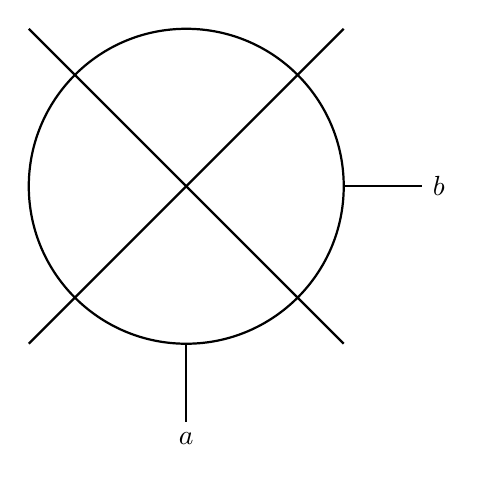
\begin{tikzpicture}
\draw[thick] (0,0) circle (2cm);
\draw[thick] (-2,-2) -- (2,2);
\draw[thick] (-2,2) -- (2,-2);
\draw[thick] (2,0) -- (3,0) node[right] {$b$};
\draw[thick] (0,-2) -- (0,-3) node[below] {$a$};
\end{tikzpicture}
\end{center}

$
\Rightarrow |y| \leq r + |a| 
$
$
\Rightarrow x^2 \leq (r + |a|)^2 
$

$
\text{Same for } y, \quad y^2 \leq (r + |b|)^2 
$

$
\forall z = (x,y) \in D_{r + \max(|a|, |b|)}
$

$
\|z\| = \sqrt{x^2 + y^2} \leq \sqrt{(r + |a|)^2 + (r + |b|)^2} 
$

$
\text{Thus if } R = \sqrt{(r + |a|)^2 + (r + |b|)^2}, \text{ the bound holds.} 
$

$
\text{\#15 is normed boundness} \equiv \text{ distance boundness.}
$

$
\text{Let } x = (x_1, x_2), y = (y_1, y_2) \in D_{r \to xy}
$

$
z_0 = (x_1, x_2)
$

$
{(x_2 - a)^2 + (y_2 - b)^2 = r^2} 
$

$
\Rightarrow d(x, (a,b)) = \sqrt{(x_1 - a)^2 + (x_2 - b)^2} \leq r 
$

$
\Rightarrow d(x, y) \leq d(x, (a,b)) + d(y, (a,b))
$

$
= \sqrt{(x_1 - a)^2 + (x_2 - b)^2} + \sqrt{(y_1 - a)^2 + (y_2 - b)^2}
$

$
\leq r + r = 2r.
$

\subsubsection*{(iii)}
Suppose that \( x \neq y \). Then \( d(x,y) \neq 0 \). Thus if we choose \(\varepsilon = d(x,y) \Rightarrow \varepsilon > 0 \), but \( d(x,y) \in \varepsilon \). (contradiction).

\medskip

(contradiction) Suppose \( x \neq y \) and so \( d(x,y) \neq 0 \). Choose \(\varepsilon > 0\) so that \(\varepsilon = d(y,x) = \frac{S}{2}\).

$
d(x,y) < \varepsilon = d\left( \frac{S}{2} \right),
$

which is a contradiction, as this implies if \( d(x,y) = S > 0 \Rightarrow d(x,y) = S < \varepsilon = \frac{S}{2} \).

$
\Rightarrow S < \frac{S}{2} \Rightarrow 2S < S.
$

Thus \( x = y \).

\subsubsection*{(iv)}
Let \((V, \| \cdot \| )\) be a normed vector space. Then let \( r > 0 \) and \( x \in V \). Then 

$
B_r^{'}(x) = \{ u \in V \mid d(x,u) < r \}
$

$
B_{r + \| x \| } (0) = \{y \in V \mid d(0,u) < r + \| x \| \}
$

\begin{center}
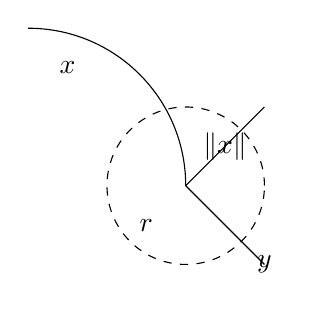
\begin{tikzpicture}
    \draw (0,0) arc (0:90:2);
    \draw (0,0) -- (1,-1);
    \draw (0,0) -- (1,1);
    \draw[dashed] (0,0) circle (1);
    \node at (-1.5,1.5) {$x$};
    \node at (1,-1) {$y$};
    \node at (-0.5,-0.5) {$r$};
    \node at (0.5,0.5) {$\| x \|$};
\end{tikzpicture}
\end{center}

Let \( y \in B_r(x) \).

$
d(0,y) \leq d(0,x) + d(x,y)
$

$
\leq \| x \| + r
$

$
\Rightarrow B_r(x) \subseteq B_{r + \| x \|}(0).
$

\subsubsection*{(v)}
Suppose \(\mathscr{S}\) is bounded. Then \(\exists M \in \mathbb{R} : \forall x \in \mathscr{S} \: \| x \| \leq M\).

(Equal to \(\exists M \in \mathbb{R} : \forall x \in \mathscr{S} \: x \in B_{\textbf{M}} (0)\))\end{document}